% This work is licensed under the Creative Commons Attribution-ShareAlike 4.0 International License.
% To view a copy of this license, visit http://creativecommons.org/licenses/by-sa/4.0/.
\documentclass[a4paper,10pt]{article}
\usepackage{fontspec} % Compile with \XeLaTeX
\usepackage{hyperxmp} % Import license metadata
\usepackage{titling} % Get the author for the metadata
\usepackage{xcolor} % Grey comments
\usepackage[colorlinks, allcolors=blue,xetex]{hyperref}
\usepackage{graphicx}
\usepackage{pgfgantt} % Gantt chart
\usepackage{natbib}
\usepackage[acronym,toc,shortcuts,nohypertypes=acronym]{glossaries} % Acronyms
\usepackage{tikz} % Charts

\bibliographystyle{apalike}

\title{Tropical forest selective logging detection through time series}
\author{Dainius Masiliūnas}

% Values copied from the license chooser, this is the only way to include it in XeTeX
\hypersetup{
    pdflicenseurl={http://creativecommons.org/licenses/by-sa/4.0/},
    pdfcopyright={This work is licensed under the Creative Commons Attribution-ShareAlike 4.0 International License.},
    pdfauthor={\theauthor}, % These are supposed to be the default but don't seem to be
    pdftitle={\thetitle},
    pdflang={en-GB}
}

% Define acronyms
\newcommand{\underletter}[1]{\textbf{#1}} % Quick toggle of underlines
\newacronym{NDVI}{NDVI}{\underletter{N}ormalised \underletter{D}ifference \underletter{V}egetation \underletter{I}ndex}
\newacronym{REDD+}{REDD+}{\underletter{R}educing \underletter{E}missions from \underletter{D}eforestation and forest \underletter{D}egradation}
\newacronym{LAI}{LAI}{\underletter{L}eaf \underletter{A}rea \underletter{I}ndex}
\newacronym{EVI}{EVI}{\underletter{E}nhaced \underletter{V}egetation \underletter{I}ndex}
\newacronym{OLI}{OLI}{\underletter{O}perational \underletter{L}and \underletter{I}mager}
\newacronym{NBR}{NBR}{\underletter{N}ormalised \underletter{B}urn \underletter{R}atio}
\newacronym{NDMI}{NDMI}{\underletter{N}ormalised \underletter{D}ifference \underletter{M}oisture \underletter{I}ndex}
\newacronym{TM}{TM}{\underletter{T}hematic \underletter{M}apper}
\newacronym{ETM+}{ETM+}{\underletter{E}nhanced \underletter{T}hematic \underletter{M}apper \underletter{Plus}}
\newacronym{WUR}{WUR}{\underletter{W}ageningen \underletter{U}niversity \& \underletter{R}esearch}
\makenoidxglossaries

% Flowchart blocks
\usetikzlibrary{shadows}
\tikzstyle{block} = [rectangle, draw, fill=white, 
    text width=8em, text centered, rounded corners, minimum height=3em]
\tikzstyle{line} = [draw, -latex']
\tikzstyle{data} = [trapezium, trapezium left angle=70, trapezium right angle=110, text centered, draw,
    text width=7em, fill=gray!30, double copy shadow, minimum height=3em]
\tikzstyle{datasingle} = [trapezium, trapezium left angle=70, trapezium right angle=110, text centered, draw,
    text width=8em, fill=gray!30]
\tikzstyle{bigdata} = [trapezium, trapezium left angle=80, trapezium right angle=100, text centered, draw,
    text width=14em, fill=gray!30, double copy shadow, minimum height=3em]

\begin{document}

\maketitle

\section{Introduction}

Selective logging is a process by which trees in a forest are cut down according to specific criteria rather than indiscriminately. This is common practice in tropical forests, where high biodiversity leads to a highly complex forest structure with trees of different sizes, shapes and properties. Trees that are interesting for logging activities are typically of a particular species or size, and tend to be spread over an area. Once a large tree is cut down, it falls on other trees. This causes a disturbance in the area, especially if only the tree stem is extracted, leaving the canopy (large branches and foliage) on top of the understory and forest floor.

Selective logging contributes to forest degradation, as per the United Nations \ac{REDD+} programme. Forests where selective logging occurs most often remain forests \citep{asner_condition_2006}, but they are disturbed, as wood from large trees is removed from the ecosystem, and succession is initiated at the points of disturbance, resulting in the replacement of mature, climax community trees with young pioneer species. This process may be part of illegal logging \citep{rutishauser_rapid_2015}, in which case the result is loss of biodiversity and lowered forest resilience. However, it could also be part of sustainable forestry practices, in which case trees are selected and logged in a way that reduces this negative impact to the forest and creates favourable conditions for succession in managed forests \citep{west_forest_2014, keller_4._2004}. Selective tree dieoff may also be caused by natural events, such as windstorms and landslides \citep{frolking_forest_2009}. In all cases, monitoring such forest degradation is a key part of the \ac{REDD+} programme. It is important to monitor such activity in order to minimise illegal logging and allow for more precise estimation of existing and historical carbon stocks \citep{piponiot_carbon_2016, pinard_simulated_2000}.

Depending on the size of the disturbance, it is possible to detect and quantify such activity from satellite imagery \citep{shimizu_using_2017, frolking_forest_2009, broadbent_recovery_2006, keller_4._2004}. That also allows for estimating the length of succession in the particular area. Precise knowledge of the recovery time after selective logging is important directly for the countries in the area for setting logging policies, as well as indirectly for climate change modelling \citep{rutishauser_rapid_2015}. However, so far such estimation has been challenging \citep{piponiot_carbon_2016} and thus it has only been performed based on chronosequences (forest plots of different timespan since logging) \citep{broadbent_recovery_2006} or extrapolated from recovery rates \citep{rutishauser_rapid_2015}. Making use of the full archive of satellite imagery to construct a time series would allow for a more precise estimate of regrowth time as well as per-tree statistics, while eliminating plot-specific effects. In addition, a system could be developed that detects such selective logging events and provides for both their near-real-time monitoring and information on whether and when selective logging has occurred in the past. This would in turn enhance the knowledge on the current and past state of tropical forests, provide information on how widespread selective logging is and help quantify its effects on the tropical forest ecosystem.

While full secondary forest regrowth after logging may take up to 125 years \citep{rutishauser_tree_2016}, the canopy closure at the selective logging site happens much faster, estimated at 6-3 months depending on the size of the disturbance \citep{broadbent_recovery_2006}. Once the canopy becomes closed, there is no more discernible difference between a logged site and a pristine forest site as seen from spaceborne optical sensors. However, knowing the precise time it takes for the canopy to close is useful, since it is an indicator of site productivity and thus is likely to correlate with biomass recovery time. In addition, knowing the location of disturbances and their canopy closure times would allow for a more accurate large-scale estimation and monitoring of biomass and carbon stocks in tropical forests by enhancing tropical forest post-logging regrowth models \citep{herault_growth_2010}. Moreover, the timespan of months rather than decades is more suitable for remote sensing applications, as it enables the use of modern sensors such as Sentinel-2 and Landsat 8 \ac{OLI} for a more accurate selective logging event detection, including near-real-time detection, as well as more precise canopy closure time estimation.
% TODO: Did anyone try to use canopy closure time as an estimate of productivity?
% TODO: Terms: canopy closure time or recovery time?
% NOTE: What about fusing sensors by using (a) common image(s) by assuming that the differences are all due to sensors, and estimating parameters for converting one to the other?
% NOTE: What makes selective logging selective is that it's small scale. So could use neighbouring pixels as a refrence of undisturbed forest rather than stable history. The problem is 1) how to determine which pixels are not affected, 2) cloud cover is a wrench in the works.

\section{Problem definition and research questions}

While satellite image time series trajectory analysis has been relatively well-established in the recent years, few studies focus on the estimation of canopy regrowth time using this technique. Most studies of tropical forest regrowth make use of chronosequences of plots with different age instead. However, time series analysis is well-suited for this purpose, because it allows detecting the disturbance time and regeneration length in a much more precise manner. In addition, time series analysis is not affected by site-specific effects, as is the case with chronosequences.

Another advantage of using satellite imagery for detecting selective logging is that it is spatially exhaustive. Satellites constantly monitor surface reflectance over the entire globe, it is not limited to a select number of test plots. Therefore a system to detect selective logging would bring information on selective logging activities in the whole Amazon rainforest, which is lacking at the moment. This is important for both \ac{REDD+} monitoring activities as well as setting local logging policy. What is more, a near-real-time selective logging monitoring system would be capable of empowering local governments to fight illegal logging more effectively. In addition, selective logging event detection, coupled with more precise estimation of canopy regrowth time, would help improve biomass estimation and carbon cycling models.

The goal of this thesis is to expand the knowledge about the extent and impact of selective logging in the Amazon rainforest by detecting selective logging events and quantifying the post-logging canopy regrowth time from satellite imagery. The research questions that the thesis will aim to answer are:

\begin{itemize}
 \item What data is required and which approach is appropriate for detecting known selective logging events from satellite imagery time series?
 \item What are the possibilities of extending this approach to detect previously unknown selective logging events?
 \item What is the canopy closure time of tropical forests in the Amazon after a selective logging event?
\end{itemize}

\section{Methods}

\subsection{Input data}

The main data used to carry out the analysis will be data from the Landsat mission archive, specifically the Collection 1 Surface Reflectance products of Landsat 5 \ac{TM}, Landsat 7 \ac{ETM+} and Landsat 8 \ac{OLI}. These sensors produce global multispectral imagery at 30 metre spatial resolution. Depending on the date at which a selective logging event happened and which Landsat satellites were active at the time, the whole history of the selected Landsat mission imagery at the selective logging location will be retrieved for time series analysis. History before the logging event is required in order to determine the stable pre-logging history that is only affected by seasonality, whereas the imagery after the logging event is needed to determine the canopy regrowth time.

Additional data from the Sentinel-2 mission may also be used in case canopy regrowth period extends into the period after the launch of Sentinel-2, or in case the spatial resolution of Landsat imagery is deemed insufficient for the task.

\subsection{Reference data}

\begin{figure}
  \centering
  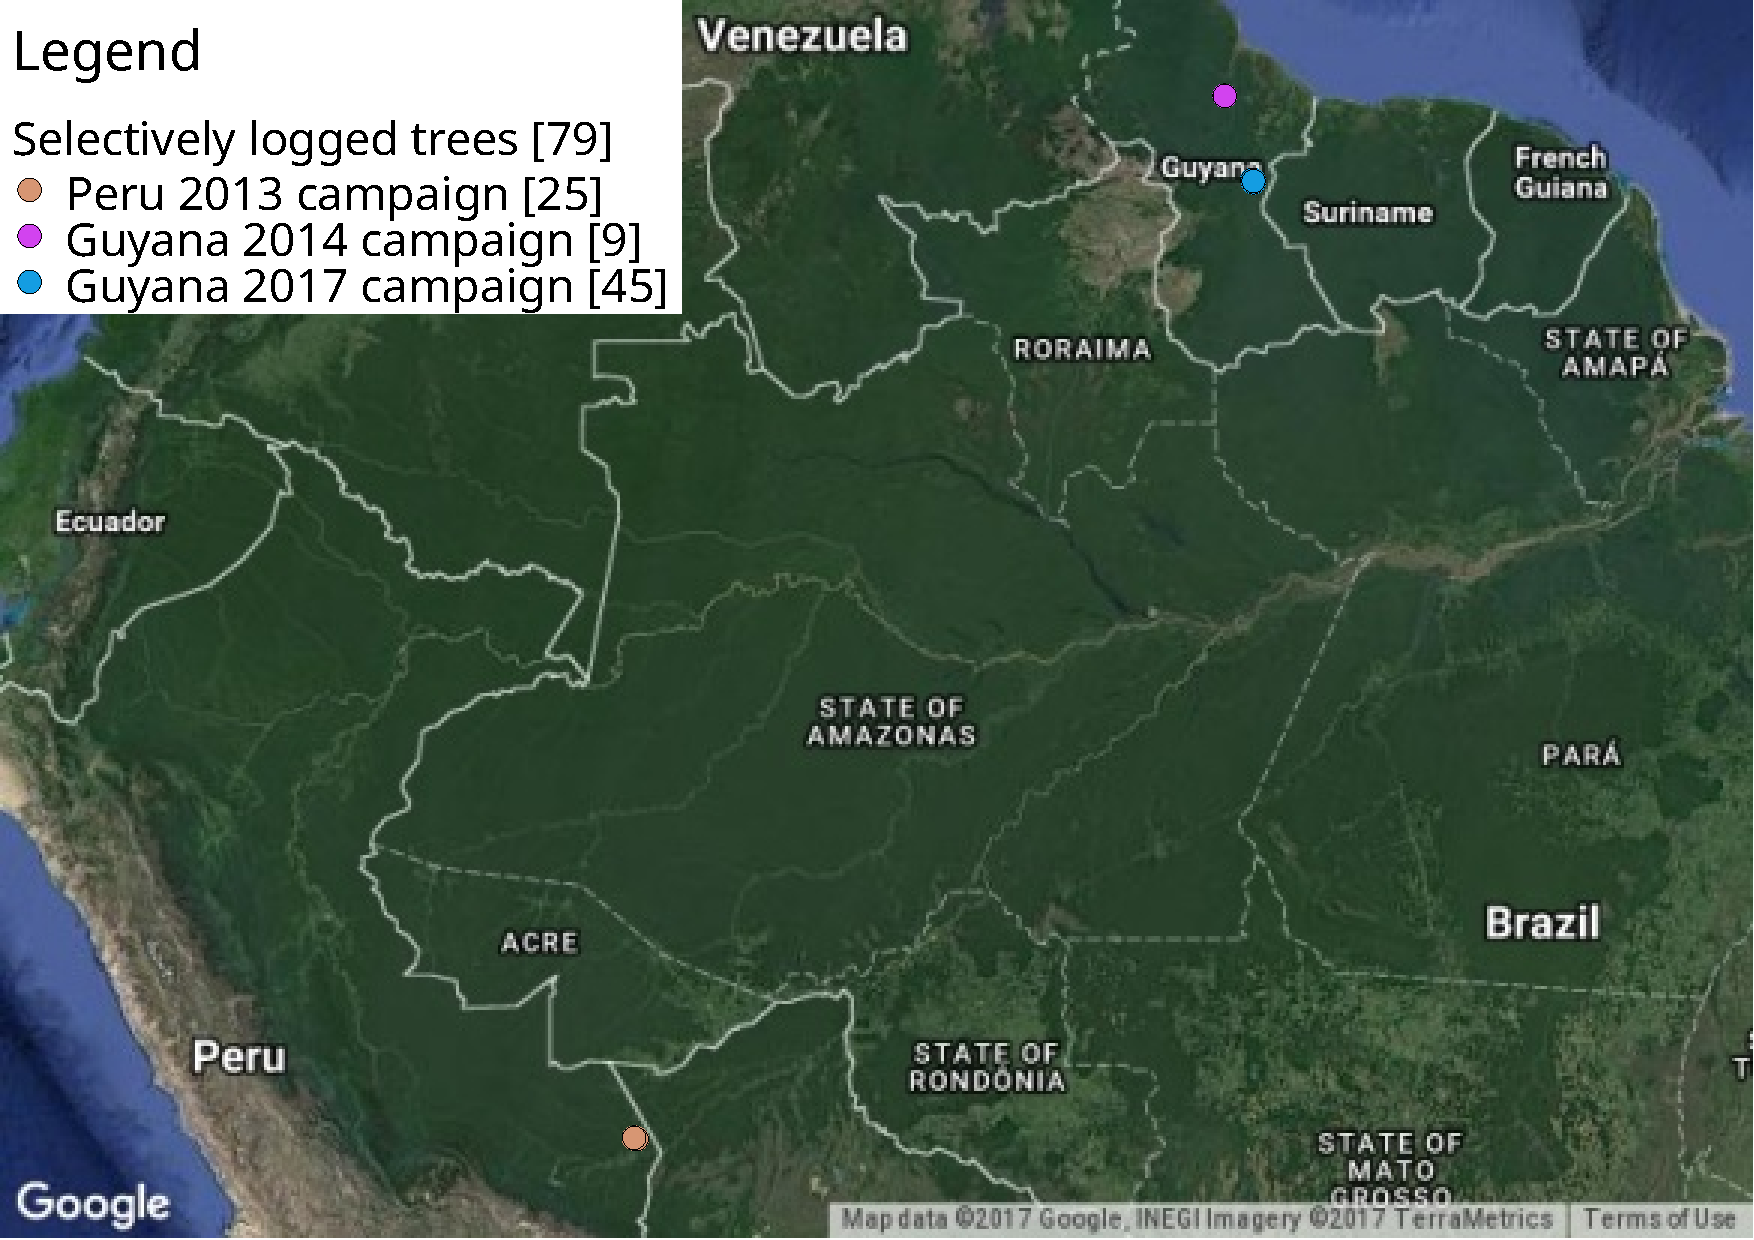
\includegraphics[width=\textwidth]{proposal-figures/AOI}
  \caption{Area of interest, with the three Lidar campaigns indicated with circles. The numbers in square brackets indicate the number of potential selective logging event locations per campaign.}
  \label{fig-aoi}
\end{figure}

In order to detect selective logging, reference data about trees that have been selectively logged is required. For this, information from the \ac{WUR} Lidar field campaigns will be used. Two field campaigns were carried out in Guyana in 2014 and 2017, and one field campaign in Peru in 2013. Lidar scans were taken at plots in which trees were in the process of being selectively logged. One Lidar scan was taken before and one after the event, with the scanning dates and scan locations registered \citep{gonzalez_de_tanago_estimation_2017}. This reference data will be used as the starting point for selective logging detection and regrowth monitoring. The locations of the campaigns is shown in figure \ref{fig-aoi}.

In addition, the data from \citet{broadbent_recovery_2006} will be used in order to directly compare the chronosequence and time series analysis methods for estimating the time of canopy closure.

\subsection{Regrowth analysis}

% TODO: Look at the best index for biomass estimation in the tropics; IDB suggests EVI, NDVI, (O/T)SAVI, NDBleaf (SWIR2-SWIR1); also NBR, TCARI/OSAVI, tasseled cap. VPI (vegetation productivity index) is a temporal measure of regrowth itself (how much NDVI deviates from yearly mean within the range, but the range needs to be big enough, which may not fit tropics), FCover would be OK but can't calculate.
% NDMI is difference between NIR and closer SWIR(1), NBR is between NIR and SWIR(2).
% Ben also suggests NDFI, but that requires endmembers (which then is better with Random Forest etc. etc.)
% Would be nice if there was an index where cloud would increase the index value. Else might need to use the same masking method as for PROBA-V
In order to determine how long it takes for the canopy to close after a selective logging event, it is necessary to obtain the time series of the pixel(s) of interest. The time series of \ac{NDVI} is most often used, but any other vegetation index or a spectral band could also be used. \ac{NDVI} is known to saturate at the higher value range compared to biophysical parameters such as \ac{LAI}, so other vegetation indices, such as \ac{EVI}, may be better suited for a more accurate estimation of canopy regrowth time. Other studies that used Landsat time series for vegetation monitoring used \ac{NBR} \citep{schneibel_assessment_2017, shimizu_using_2017}, \ac{NDMI} \citep{dutrieux_reconstructing_2016} and tasseled cap transformation greenness \citep{powell_quantification_2010}. \ac{EVI} will be used as a starting point, but other vegetation indices may also be tested, time permitting.

After the construction of the time series for every known location of selective logging, the \textit{R} packages \textit{BFAST} \citep{verbesselt_detecting_2010} and \textit{BFASTMonitor} \citep{verbesselt_near_2012} will be used to detect breaks in the time series that correspond to the logging events. Then, the package \textit{rgrowth} \citep{devries_tracking_2015} will be used to calculate the total time it takes for the time series to recover to the pre-logging state, i.e. the time it takes for the vegetation index to saturate again due to canopy closure.

This processing step will be applied to all pixels within a bounding box that incorporates all pixels within a 60 m radius of the reference data on selectively logged trees. This will be done in order to account for possible inaccuracies in the GPS field measurements, as well as to cut down on the data processing time, while still leaving enough pixels to process so as to make sure that the processing chain is generic enough to handle pixels that are not hand-picked.

\subsection{Event detection}

% TODO: Last break, or the largest break?
Once the approach for quantifying regrowth of known selective logging events is determined, it will be possible to apply this approach to a larger area in order to determine previously unknown selective logging or other disturbance events. The result of such event detection will be a raster showing the regrowth times of the last significant break in the time series. The more time it takes for the canopy to recover, the more likely the area has been affected by selective logging. In addition, another raster showing the dates at which the break happened will be made, so that it would be possible to verify what sort of disturbance the breaks represent by referring to historical data.

A schematic view of the whole processing chain is shown in figure \ref{fig-processing}.

\begin{figure}
  \centering
  \begin{tikzpicture}[node distance = 0.5cm, auto]
      % DEM
      \node [data] (l3amp) {Level 3 satellite imagery};
      \node [block, below= of l3amp] (cloud) {Cloud masking};
      \node [block, right= of cloud, fill=yellow] (bbox) {AOI bounding box calculation};
      \node [datasingle, above= of bbox] (ref) {Reference points};
      \node [block, below= of cloud, fill=yellow] (crop) {Cropping to bounding box};
      \node [block, below= of crop] (stack) {Time series stacking};
      \node [block, below= of stack] (vi) {Vegetation index calculation};
      \node [block, below= of vi] (breaks) {Time series break detection};
      \node [datasingle, below= of breaks] (break-map) {Latest significant break date map};
      \node [block, right= of breaks] (rgrowth) {Regrowth time calculation};
      \node [datasingle, below= of rgrowth] (rgrowth-map) {Regrowth time map};
      % Draw edges
      \path [line] (l3amp) -- (cloud);
      \path [line] (ref) -- (bbox);
      \path [line] (cloud) -- (crop);
      \path [line] (bbox) -- (crop);
      \path [line] (crop) -- (stack);
      \path [line] (stack) -- (vi);
      \path [line] (vi) -- (breaks);
      \path [line] (vi) -- (rgrowth);
      \path [line] (breaks) -- (break-map);
      \path [line] (rgrowth) -- (rgrowth-map);
  \end{tikzpicture}
  \caption{Proposed processing chain. Grey blocks are input and output data, rounded blocks are scripts that process the data. Scripts in yellow will only be used for initial model parameter determination and validation, not for full-tile processing. Depending on time constraints and whether it will be necessary, the time series stacking step may also involve multisensor data fusion.}
  \label{fig-processing}
\end{figure}

\subsection{Validation}

The reference data will also be used for the validation of the resulting selective logging disturbance time map. Since the approximate location and date of a selective logging event is known from the reference data, the disturbance map must correspond to the reference data. The regrowth time map will be validated by comparison with \citet{broadbent_recovery_2006} and other relevant literature. For the previously unknown selective logging detection step, the resulting map and the intermediary data will be assessed visually.

\section{Time schedule and feasibility}

\subsection{Time schedule}

\begin{figure}
  \resizebox{\textwidth}{!}{
    \begin{ganttchart}[hgrid, vgrid]{1}{20}
      \gantttitle{2017}{20} \\
      \gantttitle{{\scriptsize May}}{1} \gantttitle{June}{4} \gantttitle{July}{5} \gantttitle{August}{4}
      \gantttitle{September}{4} \gantttitle{{\scriptsize October}}{2} \\
      \gantttitle{29}{1} \gantttitle{5}{1} \gantttitle{12}{1} \gantttitle{19}{1} \gantttitle{26}{1}
      \gantttitle{3}{1} \gantttitle{10}{1} \gantttitle{17}{1} \gantttitle{24}{1} \gantttitle{31}{1}
      \gantttitle{7}{1} \gantttitle{14}{1} \gantttitle{21}{1} \gantttitle{28}{1}
      \gantttitle{4}{1} \gantttitle{11}{1} \gantttitle{18}{1} \gantttitle{25}{1}
      \gantttitle{2}{1} \gantttitle{9}{1} \\
      \ganttbar{Proposal writing}{1}{4} \\
      \ganttbar{Thesis writing}{5}{19} \\
      \ganttgroup{Analysis}{4}{17} \\
      \ganttbar{Preprocessing}{4}{8} \\
      \ganttbar{Regrowth analysis}{8}{11} \\
      \ganttbar{Multisensor fusion}{10}{14} \\
      \ganttbar{Event detection}{14}{17} \\
      \ganttgroup{Finalisation}{18}{20} \\
      \ganttbar{Presentation}{20}{20} \\
      \ganttmilestone{Thesis defence}{20}
    \end{ganttchart}
  }
  \caption{Gantt chart of the time schedule. Numbers in the third line represent the Monday of the indicated week.}
  \label{fig-gantt}
\end{figure}

The minor thesis is planned to take a total of 20 weeks to complete, 14 of which are planned to be spent on data analysis, starting from May 29 and ending on October 13, 2017. See figure \ref{fig-gantt} for more details.

\subsection{Feasibility and risks}

The proposed study requires a set of satellite and reference data. The risk of having no access to satellite data is minimal, since both the Landsat and Sentinel archives as well as their preprocessing tools are freely available on the internet. In the case of Landsat imagery, a preprocessing service is available, which provides level 3 surface reflectance data on demand. In case the preprocessing service becomes unavailable or takes too long to preprocess the data, the \textit{LEDAPS} preprocessing tool will be run manually. If Sentinel-2 data will be used, it will be necessary to run its preprocessing tool (\textit{sen2cor}) manually, as there is no preprocessing service for this data yet. In the case of reference data, the availability of the \ac{WUR} Lidar plot dataset is guaranteed since the data is public as well. However, the Bolivian plot dataset from \citet{broadbent_recovery_2006} is not guaranteed to be available on time for processing. In case it is not available, only the \ac{WUR} Lidar plot dataset will be used.

Since detection of selective logging from satellite imagery time series has not been performed in the Amazonian forests before, there are substantial risks as to whether it is feasible. Literature indicates that selectively logged sites have substantially different reflectance values compared to pristine sites \citep{broadbent_recovery_2006}, and detecting such events from Landsat data was successfully done for Asian tropical forests \citep{shimizu_using_2017}, therefore it should be possible to do so in the Amazon as well. In order to minimise this risk, the time series of multiple vegetation indices will be tested, higher resolution sensors will be tried, and multisensor fusion will be attempted in order to gain more complete time series. In the unlikely case that selective logging detection from satellite imagery is not feasible after all, the thesis will focus on which methods have been attempted and why they were insufficient in this particular case, compared to related studies that have been successful at it.

Since regrowth time quantification has not been performed on Amazon rainforest time series so far either, there is also a risk of whether that will be possible. Multisensor fusion would also help in this case, since having denser time series allows for more accurate quantification of regrowth time. Overall this risk is low, since regrowth time can also be estimated from the time between the time series break related to the logging event and the break related to the stop in regrowth and return to stable year-to-year conditions.

Given that the thesis deals with time series data, which is by nature big data, there is a risk of image processing taking a long time. This risk will be minimised by first performing processing only in the immediate area of where selective logging is known to have occurred, no more than 25 pixels per area disturbed by a logging event. The pixels will be extracted from the full tiles, and will be stored and processed separately, as to exclude all of the irrelevant data outside of the logged areas and thus speed up processing. The previously unknown logging event detection step will only be performed if there is sufficient time for processing more data, and no more than an extent of a single Landsat tile will be used for selective logging event detection purposes.

Multisensor fusion itself is a highly complex task that requires matching the reflectance values of multiple sensors together as well as over time, therefore it carries risks of feasibility and time requirements. Therefore, even though multisensor fusion would be beneficial to more precise regrowth time estimation and ease logging event detection, it will only be performed if single-sensor solutions are deemed insufficient. The workflow will first be tested on imagery from a single sensor, and only if logging event detection or regrowth time estimation fails will multisensor fusion be attempted. In addition, for some pairs of sensors, methodology for multisensor fusion has already been well-established and thus should be much simpler. For instance, Landsat TM and ETM+ data is often fused by performing preprocessing to surface reflectance values via LEDAPS.

\printnoidxglossary[type=acronym]

\bibliography{bibliography}

\end{document}
